\documentclass[runningheads]{llncs}

\usepackage[T1]{fontenc}
\usepackage[utf8]{inputenc}
\usepackage{amsmath,amssymb}
\usepackage{booktabs}
\usepackage{tabularx}
\usepackage{array}
\usepackage{float}
\usepackage{graphicx}
\usepackage{tikz}
\usepackage{pgfplots}
\usepackage{url}
\usepackage{seqsplit}
\usepackage{placeins}
\usepackage{algorithm}
\usepackage{algpseudocode}
\usetikzlibrary{arrows.meta,positioning}
\pgfplotsset{compat=1.18}
\setlength{\emergencystretch}{2em}

\begin{document}
\title{Data-Efficient Projection-Related Tuning of BioMedCLIP for Ultrasound Image--Text Retrieval Using US-365K}
\titlerunning{Projection-Related Tuning of BioMedCLIP for Ultrasound Retrieval}
\author{Bui Xuan Tung\inst{1,2}\thanks{Corresponding author: bxtung@tdu.edu.vn} \and Ma Truong Thanh\inst{1} \and Tran Viet Chau\inst{1}}
\authorrunning{B. X. Tung et al.}
\institute{Can Tho University, Can Tho City, Vietnam\\
\email{tungp2425004@gstudent.ctu.edu.vn, mtthanh@ctu.edu.vn, tvchau@ctu.edu.vn} \and
Tay Do University, Can Tho City, Vietnam\\
\email{bxtung@tdu.edu.vn}}
\maketitle
\begin{abstract}
\textbf{Purpose:} Ultrasound image--text retrieval requires alignment between sonographic appearance and textual descriptions under substantial visual variability and semantic redundancy. This study evaluates whether BioMedCLIP can be adapted to ultrasound using a constrained set of projection-related parameters rather than full-model fine-tuning, and whether improvements observed on a controlled test subset persist when retrieval is evaluated against the complete US-365K test gallery. \textbf{Approach:} We adapt BioMedCLIP using the public US-365K dataset. Most pretrained parameters are frozen; trainable parameters are selected by implementation-level name matching for \texttt{proj} or \texttt{projection}, together with the learnable \texttt{logit\_scale}. Data-efficiency experiments use 1k, 5k, 10k, and 50k training subsets with fixed 5k validation and test subsets. The selected FT-50k checkpoint is additionally evaluated on the complete usable test split. Of 71,919 original test pairs, one unreadable image is excluded, leaving 71,918 valid image--text pairs. \textbf{Results:} Recall@K is reported as a percentage. On the controlled 5k test subset, FT-50k increases I2T Recall@10 from 3.88\% to 7.60\% and T2I Recall@10 from 4.46\% to 7.90\%. On the 71,918-pair full gallery, I2T Recall@10 increases from 0.3740\% (95\% CI, 0.3320--0.4214\%) to 0.4436\% (0.3976--0.4948\%; unadjusted paired $p=0.0217$), whereas T2I Recall@10 increases from 0.4602\% (0.4134--0.5124\%) to 0.6938\% (0.6358--0.7572\%; unadjusted paired $p<0.001$). The six Recall@$K$ paired tests are exploratory and are reported without multiplicity adjustment. A complementary strict-greater rank statistic decreases from 5,806 to 2,536 positions for I2T and from 5,631 to 2,482 positions for T2I. \textbf{Conclusions:} Projection-related tuning of a largely frozen BioMedCLIP model produces measurable ultrasound-specific adaptation using 50,000 training pairs and preserves a ranking advantage when retrieval is expanded to the 71,918-item gallery. The resulting representation provides a data-efficient basis for ultrasound semantic retrieval and for subsequent expert-validated studies of clinically oriented search, report-assistance, and decision-support retrieval workflows.
\end{abstract}
\keywords{ultrasound image-text retrieval \and BioMedCLIP \and US-365K \and projection-related tuning \and contrastive learning \and medical image analysis}

\section{Introduction}

Let $\mathcal{D}=\{(x_i,t_i)\}_{i=1}^{N}$ denote paired medical images and textual descriptions, with $x_i\in\mathcal{X}$ and $t_i\in\mathcal{T}$. Vision-language learning seeks functions $f_{\theta_v}:\mathcal{X}\rightarrow\mathbb{R}^{d}$ and $g_{\theta_t}:\mathcal{T}\rightarrow\mathbb{R}^{d}$ that place a matched image-text pair close together in a shared embedding space and separate mismatched pairs. This representation supports retrieval, zero-shot recognition, and cross-modal transfer.
The same alignment problem is harder in medical imaging because image meaning depends on anatomy, acquisition conditions, and clinical context. Ultrasound adds speckle noise, acoustic shadowing, low contrast, probe dependence, and marked within-class variation. Visually similar scans can therefore have different textual findings, while similar findings can appear differently across examinations. These properties limit direct transfer from vision-language models trained outside the ultrasound domain.

CLIP established symmetric contrastive learning as a practical way to align images and text and showed strong zero-shot transfer \cite{radford2021clip}. ALIGN reached similar conclusions at larger scale with noisy image-text supervision \cite{jia2021align}. BioMedCLIP brought this idea into biomedicine by combining a Vision Transformer image encoder with a PubMedBERT text encoder and pretraining on millions of scientific image-caption pairs \cite{zhang2023biomedclip,dosovitskiy2021vit,gu2021pubmedbert}. ConVIRT, GLoRIA, MedCLIP, PMC-CLIP, and BioViL likewise showed that paired or weakly paired medical image-text data can improve representation learning and transfer \cite{zhang2020convirt,huang2021gloria,wang2022medclip,lin2023pmcclip,boecking2022biovil}. These studies provide the basis for asking how much of a pretrained biomedical representation must actually be changed for ultrasound.

Despite these advances, adapting a pretrained biomedical vision-language model to ultrasound remains a non-trivial problem. Let $P_{pre}(\mathcal{X},\mathcal{T})$ and $P_{us}(\mathcal{X},\mathcal{T})$ denote the joint image-text distributions of the pretraining corpus and the target ultrasound domain, respectively. In practice, $P_{pre}(\mathcal{X},\mathcal{T})\neq P_{us}(\mathcal{X},\mathcal{T})$, reflecting substantial differences in image characteristics, caption style, anatomical coverage, and semantic granularity. A straightforward solution is to fine-tune the entire model, $\Theta\leftarrow\Theta+\Delta\Theta$, where $\Theta$ denotes all trainable parameters. However, full-model fine-tuning incurs considerable computational cost, increases memory consumption, and often leads to overfitting when domain-specific annotated data are limited. These limitations motivate an alternative question that has received comparatively less attention: \textit{Can an ultrasound-specific multimodal representation be effectively learned by adapting only a projection-related parameter subspace while preserving the non-projection parameters of the pretrained BioMedCLIP image and text pathways?}

We treat this question as a constrained representation-learning problem. The non-projection BioMedCLIP parameters remain fixed, while projection-related parameters and the learnable similarity scale are optimized:
\begin{equation}
\min_{\Phi}\, \mathcal{L}_{CLIP}
\quad\text{s.t.}\quad
\Omega\ \text{is fixed},
\end{equation}
Here, $\Phi$ is the trainable projection-related subset, including the learnable logit scale, and $\Omega=\Theta\setminus\Phi$ contains the frozen non-projection parameters. In code, $\Phi$ is formed from parameter names containing \texttt{proj} or \texttt{projection}, together with \texttt{logit\_scale}. The experiment therefore changes the alignment subspace without retraining the whole multimodal model.
We evaluate this restricted update in three ways: cross-modal retrieval, scaling from 1k to 50k paired training samples, and transfer through zero-shot and linear-probing classification. The aim is to determine whether the update improves only pair matching or also changes the usefulness of the learned representation.

The work makes three contributions. First, it defines ultrasound adaptation as optimization over an implementation-defined projection-related subset while the remaining BioMedCLIP parameters are fixed. Second, it measures data efficiency with 1k, 5k, 10k, and 50k training pairs under the same controlled validation and test protocol. Third, it evaluates the adapted representation with retrieval, zero-shot classification, linear probing, and a separate full-gallery comparison between the original BioMedCLIP checkpoint and FT-50k. Together, these components establish a transparent parameter-efficient pathway for adapting a biomedical vision-language representation to ultrasound and for studying how the benefit changes with the amount of paired supervision.

\subsection{Related work and study positioning}

Ultrasound is particularly sensitive to acquisition geometry, probe placement, speckle, shadowing, and local anatomy. Ultrasound-CLIP addresses this domain directly through semantic-aware contrastive pretraining and structured diagnostic attributes \cite{jin2026usclip}. Our question is different: whether an existing biomedical model can be adapted by changing only projection-related parameters. This setting is relevant when full ultrasound-specific pretraining is impractical. The emphasis on acquisition physics and variability is also consistent with broader work on ultrasound signal processing and deep learning \cite{luijten2022ultrasound}.

The study also relates to parameter-efficient adaptation. Representative approaches include adapter modules, prompt and prefix tuning, and low-rank adaptation, all of which reduce the number of parameters changed during transfer \cite{houlsby2019adapters,lester2021prompt,li2021prefix,hu2022lora}. The present experiments isolate a complementary setting in which the trainable subset is selected directly from projection-related parameter names in BioMedCLIP. Structured comparisons with alternative parameter-efficient strategies are left for future work under the same data and evaluation protocol.

\section{Problem Formulation}

Let $\mathcal{X}$ denote the ultrasound image space and $\mathcal{T}$ the textual description space. We write the training data as $\mathcal{D}=\{(x_i,t_i)\}_{i=1}^{N}$, where $x_i\in\mathcal{X}$ and $t_i\in\mathcal{T}$ form the designated positive pair. Within the contrastive objective, $(x_i,t_j)$ with $i\neq j$ is treated as a negative association.


\subsection{Notation}
\label{lb-notion}
Let $f_{\Theta}:\mathcal{X}\rightarrow\mathbb{R}^{d_v}$ denote the BioMedCLIP visual pathway and let $g_{\Theta}:\mathcal{T}\rightarrow\mathbb{R}^{d_t}$ denote the BioMedCLIP text pathway. The complete model parameter set is denoted by $\Theta$. In this work, $\Theta$ is partitioned into a frozen non-projection subset $\Omega$ and a trainable projection-related subset $\Phi$, such that $\Theta=\Omega\cup\Phi$ and $\Omega\cap\Phi=\emptyset$. The implementation constructs $\Phi$ by enabling gradients for parameters whose names contain \texttt{proj} or \texttt{projection}, together with the learnable logit-scale parameter $\gamma$. All remaining parameters are fixed.

Given an image-text pair $(x_i,t_i)$, the model produces visual and textual embeddings $z_i^{v}$ and $z_i^{t}$ using $\Omega$ and $\Phi$. Both embeddings are normalized onto the unit hypersphere, namely $\hat{z}_i^{v}=z_i^{v}/\|z_i^{v}\|_2$ and $\hat{z}_i^{t}=z_i^{t}/\|z_i^{t}\|_2$. The similarity between an image embedding and a text embedding is defined as
\begin{equation}
\label{eq:similarity}
s_{ij}=\exp(\gamma)(\hat{z}_i^{v})^{\top}\hat{z}_j^{t},
\end{equation}
where larger values indicate stronger semantic consistency between the corresponding image-text pair. Unlike conventional full-model adaptation, which optimizes all parameters in $\Theta$, the proposed setting restricts optimization to the much smaller subset $\Phi$. In the reported FT-50k experiment, this subset contains 8,890,113 trainable parameters out of 195,902,721 total parameters, corresponding to 4.5380\% of the model.

\subsection{Projection-Constrained Optimization}

Let $\Theta=\Omega\cup\Phi$ denote the complete parameter set of the vision-language model, where $\Omega$ contains frozen non-projection parameters and $\Phi$ contains trainable projection-related parameters and the logit scale. The adaptation problem is formulated as
\begin{equation}
\label{eq:projection_problem}
\Phi^{*}=\arg\min_{\Phi}\mathcal L(\Phi;\Omega)
\quad\text{s.t.}\quad
\Omega\ \text{is fixed},
\end{equation}
where $\mathcal L(\Phi;\Omega)$ is defined in Section~2.4.

During projection-related adaptation, all parameters in $\Omega$ remain unchanged; optimization is confined to the trainable subset $\Phi$ and does not perform full-model fine-tuning.


\begin{proposition}[Spectral-Norm Bound for an Individual Linear Projection Component]
Let $P$ be one trainable linear projection component with weight matrix $W$. Then, for any two inputs $a_1$ and $a_2$,
\begin{equation}
\|P(a_1)-P(a_2)\|_2 \le \|W\|_2 \|a_1-a_2\|_2.
\label{eq:component_bound}
\end{equation}
In particular, if $P_v(v)=W_vv$ and $P_t(u)=W_tu$ denote linear visual and textual projection components, then
\begin{equation}
\|P_v(v_1)-P_v(v_2)\|_2 \le \|W_v\|_2 \|v_1-v_2\|_2,
\end{equation}
\begin{equation}
\|P_t(u_1)-P_t(u_2)\|_2 \le \|W_t\|_2 \|u_1-u_2\|_2.
\end{equation}
Thus, the distance expansion of each trainable linear projection component is bounded by its spectral norm.
\end{proposition}

\begin{proof}
Since $P(a)=Wa$, we have $P(a_1)-P(a_2)=W(a_1-a_2)$. By the definition of the spectral norm, $\|Wb\|_2\le \|W\|_2\,\|b\|_2$ for any vector $b$. Setting $b=a_1-a_2$ gives Equation~(\ref{eq:component_bound}). The two displayed special cases follow by substituting $P_v(v)=W_vv$ and $P_t(u)=W_tu$.
\end{proof}

This proposition is component-wise: it applies to trainable linear projection components such as attention-output or terminal projection layers. It does not describe the complete distributed subset $\Phi$ and does not constitute a global Lipschitz bound for the BioMedCLIP pathway, which also contains a convolutional patch projection, nonlinear operations, and frozen parameters.


\subsection{Learning Objective}

Based on the constrained optimization problem in (\ref{eq:projection_problem}), the objective is to learn projection-related parameters that maximize semantic alignment between paired ultrasound images and captions. Let $\mathcal{B}=\{(x_i,t_i)\}_{i=1}^{M}$ denote a mini-batch of $M$ image-text pairs. Passing each sample through the model under frozen $\Omega$ and trainable $\Phi$ yields normalized embeddings $\hat z_i^{v}$ and $\hat z_i^{t}$. Their pairwise similarity is computed as $s_{ij}=\exp(\gamma)(\hat z_i^{v})^{\top}\hat z_j^{t}$, where $\gamma$ is the learnable logit-scale parameter. Since all embeddings are normalized, $s_{ij}$ represents the scaled cosine similarity between image and text representations.
The image-to-text contrastive objective is defined as
\begin{equation}
\label{eq:i2t_loss}
\mathcal{L}_{i2t}=-\frac{1}{M}\sum_{i=1}^{M}\log\frac{\exp(s_{ii})}{\sum_{j=1}^{M}\exp(s_{ij})},
\end{equation}
which encourages each image to retrieve its paired text while suppressing mismatched samples. Likewise, the text-to-image objective is
\begin{equation}
\label{eq:t2i_loss}
\mathcal{L}_{t2i}=-\frac{1}{M}\sum_{i=1}^{M}\log\frac{\exp(s_{ii})}{\sum_{j=1}^{M}\exp(s_{ji})}.
\end{equation}
Optimizing both retrieval directions jointly enforces bidirectional semantic alignment. The overall learning objective is
\begin{equation}
\label{eq:loss}
\mathcal{L}(\Phi;\Omega)=\frac{1}{2}\left(\mathcal{L}_{i2t}+\mathcal{L}_{t2i}\right),
\end{equation}
and the optimal trainable parameters are obtained by $\Phi^{*}=\arg\min_{\Phi}\mathcal L(\Phi;\Omega)$ while $\Omega$ remains fixed. Consequently, all performance improvements arise from a constrained projection-related update rather than full-model fine-tuning.

\subsection{Evaluation Protocol and Statistical Uncertainty}
\label{sec:evaluation_formalism}

The learning objective specifies how $\Phi$ is estimated. Retrieval evaluation requires a separate definition of queries, candidates, hits, and rank. Let $\mathcal{Q}=\{q_i\}_{i=1}^{N_q}$ denote a query set and $\mathcal{G}=\{c_j\}_{j=1}^{N_g}$ a candidate gallery. For the strict index-matched protocol used in this study, each query $q_i$ has one designated paired candidate $c_i$. Let $s_{ij}$ denote the similarity between $q_i$ and $c_j$, and let $\mathcal{T}_{K}(i)$ be the set of indices returned by the top-$K$ operator. The exact-index hit indicator is
\begin{equation}
 h_i^{(K)}=\mathbb{I}\left[i\in\mathcal{T}_{K}(i)\right],
\end{equation}
and Recall@$K$ is reported in percentage units as
\begin{equation}
 \operatorname{R@K}(\%)=\frac{100}{N_q}\sum_{i=1}^{N_q} h_i^{(K)}.
 \label{eq:recall_percent}
\end{equation}
Thus, Recall@$K$ is dimensionless but is displayed on a percentage scale throughout the Results section.

To characterize global ordering independently of the top-$K$ hit count, the saved full-gallery evaluator also records the strict-greater rank
\begin{equation}
 \rho_i=1+\sum_{j=1}^{N_g}\mathbb{I}\left[s_{ij}>s_{ii}\right],
 \label{eq:strict_rank}
\end{equation}
and reports $\operatorname{MedR}=\operatorname{median}(\rho_i)$ in retrieval positions. Equation~(\ref{eq:strict_rank}) uses a best-rank convention under exact score ties: candidates whose score equals the target score are not counted ahead of the target. By contrast, Recall@$K$ is computed from the implementation-level top-$K$ operator. Because duplicated or nearly duplicated textual descriptions may induce equal or near-equal similarities, Recall@$K$ and $\operatorname{MedR}$ are treated as complementary metrics and are not algebraically converted into one another.

Two evaluation protocols are distinguished. The controlled protocol $\mathcal{P}_{5k}$ uses $N_q=N_g=5{,}000$ and is used to study the effect of training-set size. The full-gallery protocol $\mathcal{P}_{full}$ uses all $71{,}918$ valid test pairs as both query population and candidate gallery. Absolute Recall@$K$ values from $\mathcal{P}_{5k}$ and $\mathcal{P}_{full}$ are therefore not interpreted as measurements at the same retrieval difficulty.

\section{Methodology}

The implementation begins by freezing BioMedCLIP and then re-enabling parameters whose names contain \texttt{proj} or \texttt{projection}, together with \texttt{logit\_scale}. The resulting trainable subset contains 8,890,113 of 195,902,721 parameters. We therefore refer to the method as projection-related tuning; it is neither full-model fine-tuning nor final-head-only tuning.

\subsection{Overall Architecture}

Figure~\ref{fig:workflow} follows the preserved implementation. The visual trainable subset is distributed through the BioMedCLIP image pathway rather than placed only at its output: it includes the patch-embedding projection, the attention-output projection in each of 12 ViT blocks, and the final visual projection. The text transformer remains frozen outside two trainable text-projection layers. The learnable \texttt{logit\_scale} is included in the same optimization subset. Normalized image and text embeddings then form the bidirectional contrastive objective.

\begin{figure}[H]
\centering
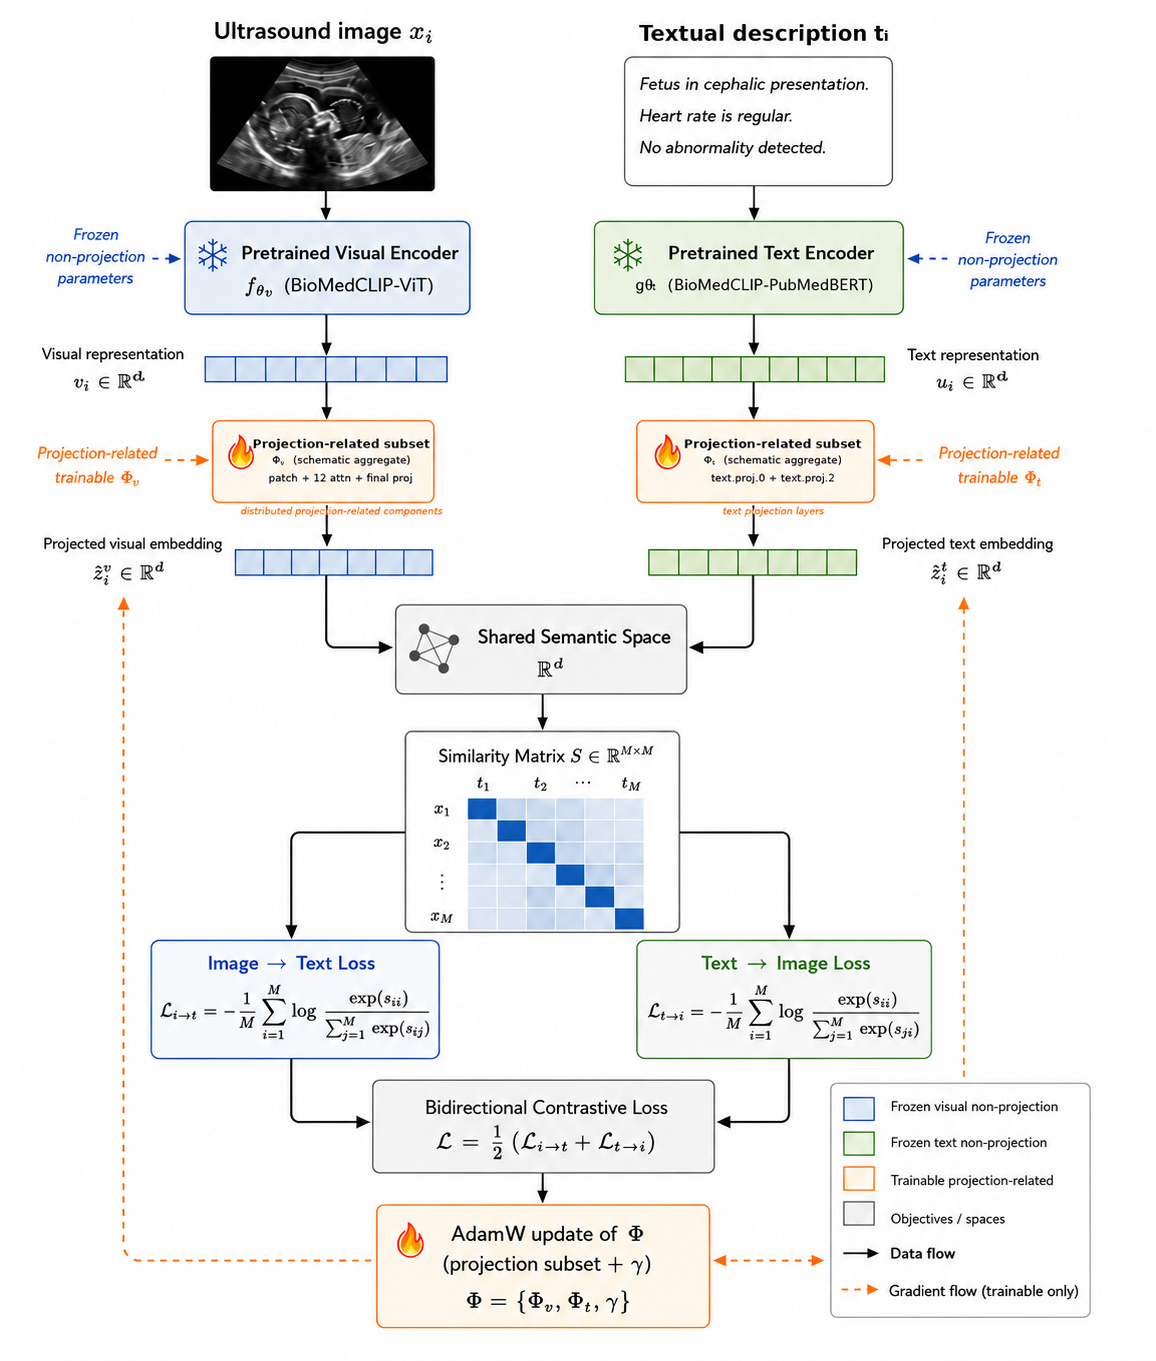
\includegraphics[width=0.76\linewidth]{Figure1_projection_related_tuning.png}
\caption{Overview of the projection-related BioMedCLIP adaptation used in this study. The orange boxes are schematic aggregates rather than terminal heads: $\Phi_v$ represents the distributed visual projection-related subset (patch-embedding projection, 12 attention-output projections, and final visual projection), $\Phi_t$ represents the two text-projection layers, and $\gamma$ is the learnable logit scale. The displayed ultrasound image and textual description are illustrative schematic inputs rather than an experimental case.}
\label{fig:workflow}
\end{figure}

\subsection{Projection-related Tuning}

Only $\Phi$ is optimized in Problem~(\ref{eq:projection_problem}). The code enables gradients for names matching \texttt{proj}, \texttt{projection}, and \texttt{logit\_scale}. The saved FT-50k checkpoint contains 30 trainable tensors: two from \texttt{visual.trunk.patch\_embed.proj}, 24 from the 12 \texttt{visual.trunk.blocks.*.attn.proj} modules, one from \texttt{visual.head.proj}, one from \texttt{text.proj.0}, one from \texttt{text.proj.2}, and the scalar \texttt{logit\_scale}. Their total is 8,890,113 parameters. Thus, the update is distributed across projection-related components rather than confined to a terminal head.

For each mini-batch $\mathcal{B}=\{(x_i,t_i)\}_{i=1}^{M}$, the implementation encodes images and texts under automatic mixed precision, normalizes the embeddings inside the symmetric contrastive loss, and updates only $\Phi$. AdamW is instantiated over parameters with \texttt{requires\_grad=True}, using learning rate $\eta=10^{-5}$ in the reported runs and weight decay $\lambda_w=0.01$. A \texttt{GradScaler} is used for the mixed-precision backward pass. Abstractly, one optimizer step is
\begin{equation}
\Phi^{(k+1)}=\mathcal{A}_{\mathrm{AdamW}}\!\left(\Phi^{(k)},
abla_{\Phi}\mathcal{L}(\Phi;\Omega);\eta,\lambda_w\right),
\end{equation}
where $\mathcal{A}_{\mathrm{AdamW}}$ acts only on $\Phi$. Hence $\Omega^{(k+1)}=\Omega^{(k)}$ for every step.


\begin{algorithm}[t]
\caption{Preserved-code projection-related adaptation and checkpoint selection}
\label{alg:projection}
\footnotesize
\begin{algorithmic}[1]
\Require Training pairs $\mathcal{D}_{tr}$; validation pairs $\mathcal{D}_{val}$; controlled test pairs $\mathcal{D}_{test}$; pretrained BioMedCLIP parameters $\Theta$; learning rate $\eta$; weight decay $\lambda_w=0.01$; epochs $E$
\Ensure Final in-memory state $\Theta_{final}$; saved best-validation checkpoint $\Theta_{best}$; best epoch $e_{best}$
\State Evaluate pretrained BioMedCLIP on $\mathcal{D}_{test}$ and store baseline metrics
\State Freeze every parameter in $\Theta$
\State Re-enable gradients only for names containing \texttt{proj} or \texttt{projection}, together with \texttt{logit\_scale}; call this subset $\Phi$ and let $\Omega=\Theta\setminus\Phi$
\State Construct AdamW over $\Phi$ with $(\eta,\lambda_w)$ and initialize AMP \texttt{GradScaler}
\State $S_{best}\leftarrow-\infty$
\For{$e=1,\ldots,E$}
    \For{all mini-batches $\mathcal{B}\subset\mathcal{D}_{tr}$}
        \State Zero AdamW gradients
        \State Under AMP, encode images/texts and compute $s_{ij}=\exp(\gamma)(\hat z_i^v)^\top\hat z_j^t$
        \State Compute $\mathcal{L}_{i2t}$ and $\mathcal{L}_{t2i}$ using Eqs.~(\ref{eq:i2t_loss})--(\ref{eq:t2i_loss}); set $\mathcal L\leftarrow\tfrac12(\mathcal{L}_{i2t}+\mathcal{L}_{t2i})$
        \State Scale $\mathcal L$, backpropagate through $\Phi$, perform AdamW step, and update scaler
    \EndFor
    \State Evaluate $\mathcal{D}_{val}$
    \State $S_e\leftarrow \operatorname{R@10}_{i2t}+\operatorname{R@10}_{t2i}$
    \If{$S_e>S_{best}$}
        \State $S_{best}\leftarrow S_e$; $e_{best}\leftarrow e$; $\Theta_{best}\leftarrow\Theta$
        \State Save \texttt{best\_model.pt} containing \texttt{model.state\_dict()}, $e$, and \texttt{valid\_metrics}
    \EndIf
\EndFor
\State $\Theta_{final}\leftarrow\Theta$
\State Evaluate $\Theta_{final}$ on $\mathcal{D}_{test}$ and store \texttt{test\_after\_finetune\_metrics.json}
\State \Return $\Theta_{final},\Theta_{best},e_{best}$
\end{algorithmic}
\end{algorithm}

The preserved training source follows this procedure. The test-set baseline is computed before adaptation but is not used in optimization or checkpoint selection. The validation score is the sum of I2T and T2I Recall@10. For FT-50k, the archived validation scores select $e_{best}=2$; the controlled 5,000-pair result is the final epoch-3 in-memory state, whereas the 71,918-pair full-gallery evaluation reloads the saved epoch-2 checkpoint. The checkpoint stores the complete model state, epoch number, and validation metrics; because $\Omega$ is fixed, differences between adapted states arise from $\Phi$.

\subsection{Inference}

At inference, an ultrasound image and each candidate text are mapped to normalized embeddings and ranked using the similarity in (\ref{eq:similarity}). The same embedding space is reused for zero-shot classification and linear probing. These downstream tests therefore measure the representation produced by the projection-related update while the non-projection parameters remain fixed.


\section{Dataset and Preprocessing}

Experiments use the public US-365K dataset \cite{jin2026usclip}, containing 364,365 ultrasound image-text records. We refer to the text as curated captions or textual descriptions rather than assuming clinical-report provenance. The released split contains 218,402 training, 74,044 validation, and 71,919 test records. Preprocessing indexes image paths, matches them to metadata, and prepares records for subset sampling.

The preserved preparation script first indexes all 364,365 image files and merges the released metadata, then generates 1k, 5k, 10k, and 50k training subsets by separate calls to Python \texttt{random.sample} after resetting \texttt{random.seed(42)} for each requested size. The subsets are therefore deterministic but are not assumed to form a strictly nested sequence. The same script generates one deterministic 5,000-pair validation subset and one 5,000-pair controlled test subset. Every training size is evaluated with that same controlled validation/test protocol. We then evaluate the BioMedCLIP baseline and the saved FT-50k checkpoint on the complete usable test gallery. One image could not be decoded by the full-gallery evaluator and was removed with its paired text from both retrieval directions; The full-gallery evaluation therefore uses 71,918 valid pairs as both queries and candidates.

Images are processed using the preprocessing associated with the released BioMedCLIP checkpoint, including resizing and checkpoint-specific normalization. Text descriptions are tokenized and truncated using the corresponding BioMedCLIP tokenizer according to the model context length \cite{zhang2023biomedclip}. No test-set pair is used for optimization or checkpoint selection.

For downstream classification, the structured \texttt{Body\_system\_level} and \texttt{Organ\_level} metadata are adopted as target labels, with the organ-level task restricted to the 20 most frequent organ categories in the training set. These experiments probe whether the adapted embedding captures anatomy-related structure that can support subsequent ultrasound semantic retrieval, report-assistance, and expert-validated decision-support studies.

\section{Experimental Setup}

The controlled training-scale experiments were run on a single NVIDIA GeForce RTX 4090 GPU. Preserved run information records PyTorch 2.2.0+cu121 and Transformers 4.41.2; the NVIDIA driver was 570.172.08 with driver-reported CUDA capability 12.8. The preserved requirements file lists \texttt{open\_clip\_torch} but does not pin its version. Training used batch size 16, four data-loading workers, AdamW with learning rate $10^{-5}$ and weight decay 0.01, and CUDA automatic mixed precision with \texttt{GradScaler}. The 5k, 10k, and 50k settings were trained for three epochs; the 1k setting was trained for one epoch and is treated as a small-data reference rather than a matched optimization-budget comparison. After every epoch, checkpoint selection used $S_e=\operatorname{R@10}_{i2t}+\operatorname{R@10}_{t2i}$ on the fixed validation subset. The training script saved \texttt{best\_model.pt} only when $S_e$ improved, and after the final epoch it evaluated the current in-memory model on the controlled test subset. For FT-50k, the saved checkpoint is epoch 2, whereas the 5,000-pair FT-50k row in Table~\ref{tab:retrieval} is the epoch-3 \texttt{test\_after\_finetune} state. The full-gallery evaluation in Tables~\ref{tab:fulltest_recall} and~\ref{tab:fulltest_rank} loads the unchanged epoch-2 FT-50k checkpoint (SHA256 \texttt{\seqsplit{3b7cb059523804c75cbbfc5a3ca16ad43c7910ea4f66c348f7968a64c6e1799f}}), uses batch size 256, 16 data-loading workers, and retrieval chunks of 4096 on one NVIDIA A100-SXM4-80GB GPU; no optimization is performed during this evaluation.

\begin{table}[t]
\scriptsize
\caption{Experimental configuration.}
\label{tab:config}
\centering
\begin{tabularx}{\linewidth}{@{}p{0.33\linewidth}X@{}}
\toprule
\textbf{Item} & \textbf{Setting} \\
\midrule
Backbone & BioMedCLIP \\
Trainable modules & Patch-embedding projection; 12 visual attention-output projections; final visual projection; two text-projection layers; logit scale \\
Frozen modules & All non-projection BioMedCLIP parameters \\
Trainable parameters & \textbf{8,890,113 / 195,902,721 (4.5380\%)} \\
Optimizer / learning rate / weight decay & AdamW / 1e-5 / 0.01 \\
Precision / gradient scaling & CUDA AMP / \texttt{GradScaler} \\
Batch size / workers & 16 / 4 \\
Retrieval train sizes & 1k, 5k, 10k, 50k \\
Retrieval validation/test & 5,000 / 5,000 pairs for the main training-scale comparison \\
Full-gallery evaluation & \textbf{71,918 valid pairs} for baseline and saved FT-50k checkpoint \\
Classification tasks & Body-system and top-20 organ labels \\
Evaluation modes & Retrieval, zero-shot, linear probing \\
Controlled-training hardware & Single NVIDIA GeForce RTX 4090 GPU \\
Full-gallery hardware & Single NVIDIA A100-SXM4-80GB GPU \\
\bottomrule
\end{tabularx}
\end{table}

\subsection{Retrieval, zero-shot, and linear probing}

Retrieval is evaluated using Recall@1, Recall@5, and Recall@10 for both image-to-text and text-to-image directions according to Equations~(\ref{eq:recall_percent})--(\ref{eq:strict_rank}). All Recall@K values are reported as percentages (\%), whereas rank-based metrics are reported in retrieval positions. Wilson intervals, paired full-gallery McNemar tests, and bootstrap median-rank intervals follow Section~\ref{sec:evaluation_formalism}. The preserved downstream script loads either the original BioMedCLIP model or the saved FT-50k best checkpoint. Zero-shot classification uses prompts of the form ``an ultrasound image of [class]'' and predicts the class with the highest normalized image--text similarity. Body-system evaluation uses all body-system classes observed in the 50k training subset; organ evaluation uses the 20 most frequent organ classes. Linear probing extracts normalized image embeddings from the 50k training subset and fits scikit-learn logistic regression with \texttt{solver=saga}, \texttt{class\_weight=balanced}, and \texttt{max\_iter=1000}. Classification is evaluated by accuracy, macro-F1, and weighted-F1. Reported controlled retrieval test values use the final training state from each run, while the FT-50k downstream classification uses the saved best-validation checkpoint. The classification results are retained as secondary descriptive representation analyses because the archived project does not contain the original per-sample prediction vectors needed for paired uncertainty analysis.

\section{Results and Discussion}
\subsection{Image--text retrieval}

\begin{table}[t]
\caption{Controlled retrieval performance on the fixed 5,000-pair test subset. Recall values are reported as percentages. The FT-50k row corresponds to the final epoch-3 training state; boldface highlights the strongest controlled result.}
\label{tab:retrieval}
\centering
\scriptsize
\setlength{\tabcolsep}{3.5pt}
\resizebox{\linewidth}{!}{%
\begin{tabular}{@{}lrrrrrrr@{}}
\toprule
\textbf{Model} & \textbf{Train} & \textbf{I2T R@1 (\%)} & \textbf{I2T R@5 (\%)} & \textbf{I2T R@10 (\%)} & \textbf{T2I R@1 (\%)} & \textbf{T2I R@5 (\%)} & \textbf{T2I R@10 (\%)} \\
\midrule
Base & 0 & 0.42 & 2.16 & 3.88 & 0.62 & 2.60 & 4.46 \\
FT1k & 1,000 & 0.28 & 1.62 & 2.94 & 0.48 & 2.70 & 4.82 \\
FT5k & 5,000 & 0.48 & 2.24 & 4.68 & 0.74 & 3.02 & 5.50 \\
FT10k & 10,000 & 0.62 & 3.02 & 5.16 & 0.82 & 3.86 & 6.62 \\
\textbf{FT50k} & \textbf{50,000} & \textbf{0.76} & \textbf{3.86} & \textbf{7.60} & \textbf{0.92} & \textbf{4.40} & \textbf{7.90} \\
\bottomrule
\end{tabular}%
}
\end{table}

Table~\ref{tab:retrieval} shows the controlled 5,000-pair comparison. The 1k model is inconsistent: I2T R@10 falls from 3.88\% to 2.94\%, while T2I R@10 rises only from 4.46\% to 4.82\%. From 5k onward, the trend is more stable. With 50k training pairs, I2T R@10 is 7.60\% (95\% Wilson CI, 6.90--8.37\%) versus 3.88\% (3.38--4.45\%) for the baseline, and T2I R@10 is 7.90\% (7.18--8.68\%) versus 4.46\% (3.92--5.07\%). These intervals describe uncertainty over the fixed test queries. The controlled experiment establishes the data-scaling trend, which is then tested separately under the full 71,918-item gallery.

We next used all 71,918 usable test pairs. Under the strict exact-index protocol in Table~\ref{tab:fulltest_recall}, FT-50k is numerically higher at every reported Recall@$K$. The unadjusted paired $p$-values are $0.0217$ for I2T R@10 and $<0.001$ for T2I R@5 and T2I R@10; the R@1 differences and I2T R@5 are not distinguishable under the same paired test. Across the six exploratory Recall tests, the Bonferroni reference threshold is $0.0083$, so the two T2I findings remain below that familywise threshold whereas I2T R@10 is nominal only. I2T R@10 changes from 0.3740\% (95\% CI, 0.3320--0.4214\%) to 0.4436\% (0.3976--0.4948\%), and T2I R@10 from 0.4602\% (0.4134--0.5124\%) to 0.6938\% (0.6358--0.7572\%), corresponding to relative increases of 18.6\% and 50.8\%.

The rank summary in Table~\ref{tab:fulltest_rank} gives the same comparison from a different angle. Median I2T rank moves from 5,806 positions (bootstrap 95\% CI, 5,721--5,888) to 2,536 (2,501--2,576), while median T2I rank moves from 5,631 (5,545--5,718) to 2,482 (2,437--2,527). Because this statistic uses the best-rank convention for exact ties, we use it only as a global ordering measure and not as a reconstruction of top-$K$ hits.

\begin{table}[t]
\caption{Full-gallery exact-index Recall@$K$ on 71,918 valid US-365K test pairs. Values are percentages with 95\% Wilson confidence intervals. The paired $p$-value is from an exact McNemar test on the same test queries. Relative change is computed with respect to the BioMedCLIP baseline. The six paired Recall tests are exploratory and unadjusted; boldface highlights findings that remain below the Bonferroni reference threshold $0.0083$.}
\label{tab:fulltest_recall}
\centering
\scriptsize
\setlength{\tabcolsep}{3.8pt}
\begin{tabular}{@{}lcccc@{}}
\toprule
\textbf{Metric} & \textbf{Baseline, \% (95\% CI)} & \textbf{FT-50k, \% (95\% CI)} & \textbf{Relative change} & \textbf{Paired $p$} \\
\midrule
I2T R@1 & 0.0445 (0.0315--0.0628) & 0.0459 (0.0327--0.0644) & +3.1\% & 1.000 \\
I2T R@5 & 0.2044 (0.1739--0.2402) & 0.2155 (0.1842--0.2522) & +5.4\% & 0.655 \\
I2T R@10 & 0.3740 (0.3320--0.4214) & 0.4436 (0.3976--0.4948) & +18.6\% & 0.0217 \\
T2I R@1 & 0.0542 (0.0397--0.0741) & 0.0695 (0.0527--0.0916) & +28.2\% & 0.278 \\
\textbf{T2I R@5} & 0.2378 (0.2047--0.2761) & \textbf{0.3574 (0.3163--0.4037)} & \textbf{+50.3\%} & \textbf{$<0.001$} \\
\textbf{T2I R@10} & 0.4602 (0.4134--0.5124) & \textbf{0.6938 (0.6358--0.7572)} & \textbf{+50.8\%} & \textbf{$<0.001$} \\
\bottomrule
\end{tabular}
\end{table}

\begin{table}[t]
\caption{Full-gallery strict-greater rank on 71,918 valid US-365K test pairs. Rank is reported in retrieval positions using Equation~(\ref{eq:strict_rank}); lower is better. Confidence intervals are from 2,000 nonparametric bootstrap resamples of query indices; boldface highlights the FT-50k rank reductions.}
\label{tab:fulltest_rank}
\centering
\scriptsize
\setlength{\tabcolsep}{5.0pt}
\begin{tabular}{@{}lccc@{}}
\toprule
\textbf{Metric (positions)} & \textbf{Baseline (95\% CI)} & \textbf{FT-50k (95\% CI)} & \textbf{Relative change} \\
\midrule
I2T median rank $\downarrow$ & 5,806 (5,721--5,888) & \textbf{2,536 (2,501--2,576)} & \textbf{-56.3\%} \\
T2I median rank $\downarrow$ & 5,631 (5,545--5,718) & \textbf{2,482 (2,437--2,527)} & \textbf{-55.9\%} \\
\bottomrule
\end{tabular}
\end{table}







\subsection{Zero-shot and linear probing classification}
A secondary representation check uses zero-shot and linear-probing classification. Body-system linear-probing accuracy changes from 60.12\% to 63.32\%, with weighted-F1 moving from 60.62\% to 63.75\%. Organ-level zero-shot accuracy changes from 43.22\% to 48.59\%, and linear-probing weighted-F1 from 52.90\% to 54.76\%. The organ-level zero-shot change is consistent with better alignment between image features and class-name prompts. Training loss also decreases over three epochs for the 5k, 10k, and 50k runs, ending at 1.2013, 0.9770, and 0.4940; we use these losses only as an optimization check.



\subsection{Retrieval error analysis}

Exact-index discrimination remains the main challenge in the controlled 5k gallery. FT50k raises I2T R@10 from 3.88\% to 7.60\% and T2I R@10 from 4.46\% to 7.90\%, but many designated pairs remain outside the top 10 because visually similar ultrasound examinations can share semantically similar captions. The 1k run provides a useful negative control: I2T R@10 falls to 2.94\%, whereas T2I R@10 changes only to 4.82\%. The improvement is therefore not automatic; the restricted projection update still requires sufficient paired ultrasound supervision. The downstream classification results provide a complementary representation-level check, with body-system linear-probing accuracy increasing from 60.12\% to 63.32\% and organ-level zero-shot accuracy from 43.22\% to 48.59\%.

\subsection{Discussion}

Performance depends on the amount of paired ultrasound data. The 1k run is unstable, while most retrieval measures improve from 5k through 50k. This pattern is consistent with BioMedCLIP already containing useful biomedical semantics but still requiring enough ultrasound pairs to reorganize cross-modal alignment.

Taken together, these results answer the research question posed in the Introduction: under the evaluated protocol, ultrasound-specific multimodal alignment improves when the projection-related parameter subset is adapted while the non-projection BioMedCLIP parameters remain fixed, with the clearest gains observed as paired ultrasound supervision increases.

\subsection{Limitations and Future Work}

The present study focuses on a controlled evaluation of projection-related BioMedCLIP adaptation using the public US-365K dataset. Although US-365K is large and covers diverse ultrasound content, evaluation on an independent external dataset would provide stronger evidence of generalization across institutions, scanner vendors, acquisition protocols, and reporting styles. Future work will therefore extend the same framework to multi-center and cross-device ultrasound datasets, with particular attention to performance shifts under different acquisition conditions.

The full-gallery experiment compares the original BioMedCLIP checkpoint with one selected FT-50k checkpoint. The current Wilson intervals, paired McNemar tests, and bootstrap rank intervals characterize uncertainty across the fixed test queries, whereas variability across independent optimization runs remains to be examined. A natural extension is to repeat the full-gallery experiment across multiple random seeds and training-set sizes and to report both query-level and seed-level uncertainty. This will provide a more complete estimate of the stability of projection-related adaptation.

Finally, the present experiments characterize \textbf{ultrasound representation adaptation and cross-modal retrieval ranking}. These results provide a technical basis for subsequent task-specific validation, external evaluation, and prospective studies. Future work will examine whether the improved multimodal representation can support clinically oriented tasks such as semantic search, decision-support retrieval, and report-related workflows under appropriate expert validation.

\section{Conclusion}

Within the evaluated protocol, the experiments answer the research question in the affirmative. We evaluated projection-related tuning of BioMedCLIP on US-365K with 8,890,113 of 195,902,721 parameters trainable (4.5380\%). The trainable subset is defined by \texttt{proj}/\texttt{projection} name matching and \texttt{logit\_scale}. Retrieval improves from 5k to 50k training pairs in the controlled 5,000-pair experiment, and the full-gallery test checks whether the selected FT-50k checkpoint retains that advantage under a much larger candidate set.

On 71,918 valid test pairs, I2T R@10 changes from 0.3740\% to 0.4436\% (18.6\% relative; unadjusted paired $p=0.0217$, nominal across six exploratory Recall tests), and T2I R@10 from 0.4602\% to 0.6938\% (50.8\% relative; unadjusted paired $p<0.001$, below the Bonferroni reference threshold $0.0083$). Strict-greater median rank changes from 5,806 to 2,536 positions for I2T and from 5,631 to 2,482 for T2I. Together with the controlled data-scaling experiment, these results show that a restricted projection-related update can reorganize ultrasound image--text similarity while preserving most pretrained BioMedCLIP parameters. The next stage is to extend this evidence through multi-seed experiments, protocol-harmonized retrieval, semantic relevance criteria, external datasets, and clinically oriented expert validation.

\section*{Data, Code, and Materials Availability}

US-365K is publicly available from the Hugging Face dataset hub at \url{https://huggingface.co/datasets/JJY-0823/US-365K}, and the pretrained BioMedCLIP checkpoint is available at \url{https://huggingface.co/microsoft/BiomedCLIP-PubMedBERT_256-vit_base_patch16_224} \cite{zhang2023biomedclip}. The source image archive is not redistributed. The code, evaluation outputs, reproducibility manifests, and reviewer-verification materials accompanying this study are available at \url{https://github.com/bxtung-hub/us365k-biomedclip-reproducibility}. The repository contains the preserved preparation, BioMedCLIP training, and downstream-evaluation scripts, together with requirements, retrieval summaries, statistical outputs, and provenance records. The FT-50k checkpoint used for the full-gallery analysis is identified by SHA256 \texttt{\seqsplit{3b7cb059523804c75cbbfc5a3ca16ad43c7910ea4f66c348f7968a64c6e1799f}}.

The supplementary audit preserves the full-gallery evaluation outputs, statistical-audit files, checkpoint identifiers, and regenerated deterministic subset manifests used to trace the reported results.

\section*{Declarations}
The authors declare that they have no competing interests related to this work. No external funding was reported for this study. This study used the publicly available US-365K dataset and involved no direct interaction with human participants.

\begin{thebibliography}{16}
\scriptsize

\bibitem{radford2021clip}
Radford, A., Kim, J.W., Hallacy, C., et al.: Learning transferable visual models from natural language supervision. In: Proceedings of the 38th International Conference on Machine Learning (ICML), pp. 8748--8763 (2021)

\bibitem{jia2021align}
Jia, C., Yang, Y., Xia, Y., et al.: Scaling up visual and vision-language representation learning with noisy text supervision. In: Proceedings of the 38th International Conference on Machine Learning (ICML), pp. 4904--4916 (2021)

\bibitem{zhang2023biomedclip}
Zhang, S., Xu, Y., Usuyama, N., et al.: A multimodal biomedical foundation model trained from fifteen million image-text pairs. NEJM AI 2(1), AIoa2400640 (2025)

\bibitem{dosovitskiy2021vit}
Dosovitskiy, A., Beyer, L., Kolesnikov, A., et al.: An image is worth 16x16 words: Transformers for image recognition at scale. In: International Conference on Learning Representations (ICLR) (2021)

\bibitem{gu2021pubmedbert}
Gu, Y., Tinn, R., Cheng, H., et al.: Domain-specific language model pretraining for biomedical natural language processing. ACM Transactions on Computing for Healthcare 3(1), 1--23 (2021)

\bibitem{zhang2020convirt}
Zhang, Y., Jiang, H., Miura, Y., Manning, C.D., Langlotz, C.P.: Contrastive learning of medical visual representations from paired images and text. arXiv preprint arXiv:2010.00747 (2020)

\bibitem{huang2021gloria}
Huang, S.C., Shen, L., Lungren, M.P., Yeung, S.: GLoRIA: A multimodal global-local representation learning framework for label-efficient medical image recognition. In: Proceedings of the IEEE/CVF International Conference on Computer Vision (ICCV), pp. 3942--3951 (2021)

\bibitem{wang2022medclip}
Wang, Z., Wu, Z., Agarwal, D., Sun, J.: MedCLIP: Contrastive learning from unpaired medical images and text. arXiv preprint arXiv:2210.10163 (2022)

\bibitem{lin2023pmcclip}
Lin, W., Zhao, Z., Zhang, X., et al.: PMC-CLIP: Contrastive language-image pre-training using biomedical documents. arXiv preprint arXiv:2303.07240 (2023)

\bibitem{boecking2022biovil}
Boecking, B., Usuyama, N., Bannur, S., et al.: Making the most of text semantics to improve biomedical vision-language processing. arXiv preprint arXiv:2204.09817 (2022)

\bibitem{jin2026usclip}
Jin, J., Chai, H., Huang, X., et al.: Ultrasound-CLIP: Semantic-aware contrastive pre-training for ultrasound image-text understanding. In: IEEE/CVF Conference on Computer Vision and Pattern Recognition (CVPR), pp. 6962--6971 (2026)

\bibitem{luijten2022ultrasound}
Luijten, B., Chennakeshava, N., Eldar, Y.C., Mischi, M., van Sloun, R.J.G.: Ultrasound signal processing: From models to deep learning. arXiv preprint arXiv:2204.04466 (2022)


\bibitem{houlsby2019adapters}
Houlsby, N., Giurgiu, A., Jastrzebski, S., et al.: Parameter-efficient transfer learning for NLP. In: Proceedings of the 36th International Conference on Machine Learning (ICML), pp. 2790--2799 (2019)

\bibitem{lester2021prompt}
Lester, B., Al-Rfou, R., Constant, N.: The power of scale for parameter-efficient prompt tuning. In: Proceedings of the 2021 Conference on Empirical Methods in Natural Language Processing (EMNLP), pp. 3045--3059 (2021)

\bibitem{li2021prefix}
Li, X.L., Liang, P.: Prefix-tuning: Optimizing continuous prompts for generation. In: Proceedings of the 59th Annual Meeting of the Association for Computational Linguistics and the 11th International Joint Conference on Natural Language Processing (ACL-IJCNLP), pp. 4582--4597 (2021)

\bibitem{hu2022lora}
Hu, E.J., Shen, Y., Wallis, P., et al.: LoRA: Low-rank adaptation of large language models. In: International Conference on Learning Representations (ICLR) (2022)

\end{thebibliography}

\end{document}
